\section{U-boot}
% ----------
\subsection{Compilation}
Configuration d'u-boot : \verb!make uboot-menuconfig!.
\begin{enumerate}
    \item \verb!make uboot-rebuild! (verbose: ajout \verb+V=1+)
    \item supprimer les fichiers puis \verb!make!
\end{enumerate}
La configuration de u-boot est stockée dans \verb!/buildroot/output/build/[version].config!
\subsubsection{Amélioration sécurité}
L'option \verb!-fstack-protector-all! (Makefile) ajoute des vérifications contre les buffer overflows (e.g. stack smashing attack).

Concrétement ajout d'une variable de garde (canary). Si modifié lors de l'éxécution d'un morceau de code $\Rightarrow$ dépassement dans le stack $\Rightarrow$ appel de la fonction \verb!__stack_chk_fail()!

Peut être statique (valeur fixe) ou dynamique (généré à la volée à chaque exécution de code par une fonction de hachage).

\subsubsection{Strip exécutable}
\verb+strip+ sur un fichier ELF (Executable and Linkable Format) supprime les symboles de débogage et les sections inutiles d'un fichier exécutable.

Cmde complète : \verb+aarch64-linux-strip u-boot+
% ----------
\subsection{Commandes u-boot}
\begin{table}[H]
\begin{tabular}{|l|l|}
    \hline
    \verb!boot!     & boot en exécutant le fichier \verb+boot.scr+\\
    \verb!booti!    & boot arm64 Linux Image\\
    \verb!ext2load! & load binary file from ext2 Filesystem\\
    \verb!ex2ls!    & list files in a directory (default: \verb!\!)\\
    \verb!fatinfo!  & print info about FAT system\\
    \verb!fatload!  & load binary file from FAT Filesystem\\
    \verb!printenv! & print environment variables\\
    \verb!mmc!      & access memory card MMC/SD\\
    \hline
\end{tabular}
\end{table}

Avec les commandes présentes dans \verb!boot.cmd!, on indique l'emplacement dans la ram de \verb!Image! et \verb!nanopi-neo-plus.dtb!\\
Lors du démarrage, le Secondary Program Loader (sunxi-spl) va charger le fichier \verb!u-boot.itb!
\begin{figure}[H]
    \centering
    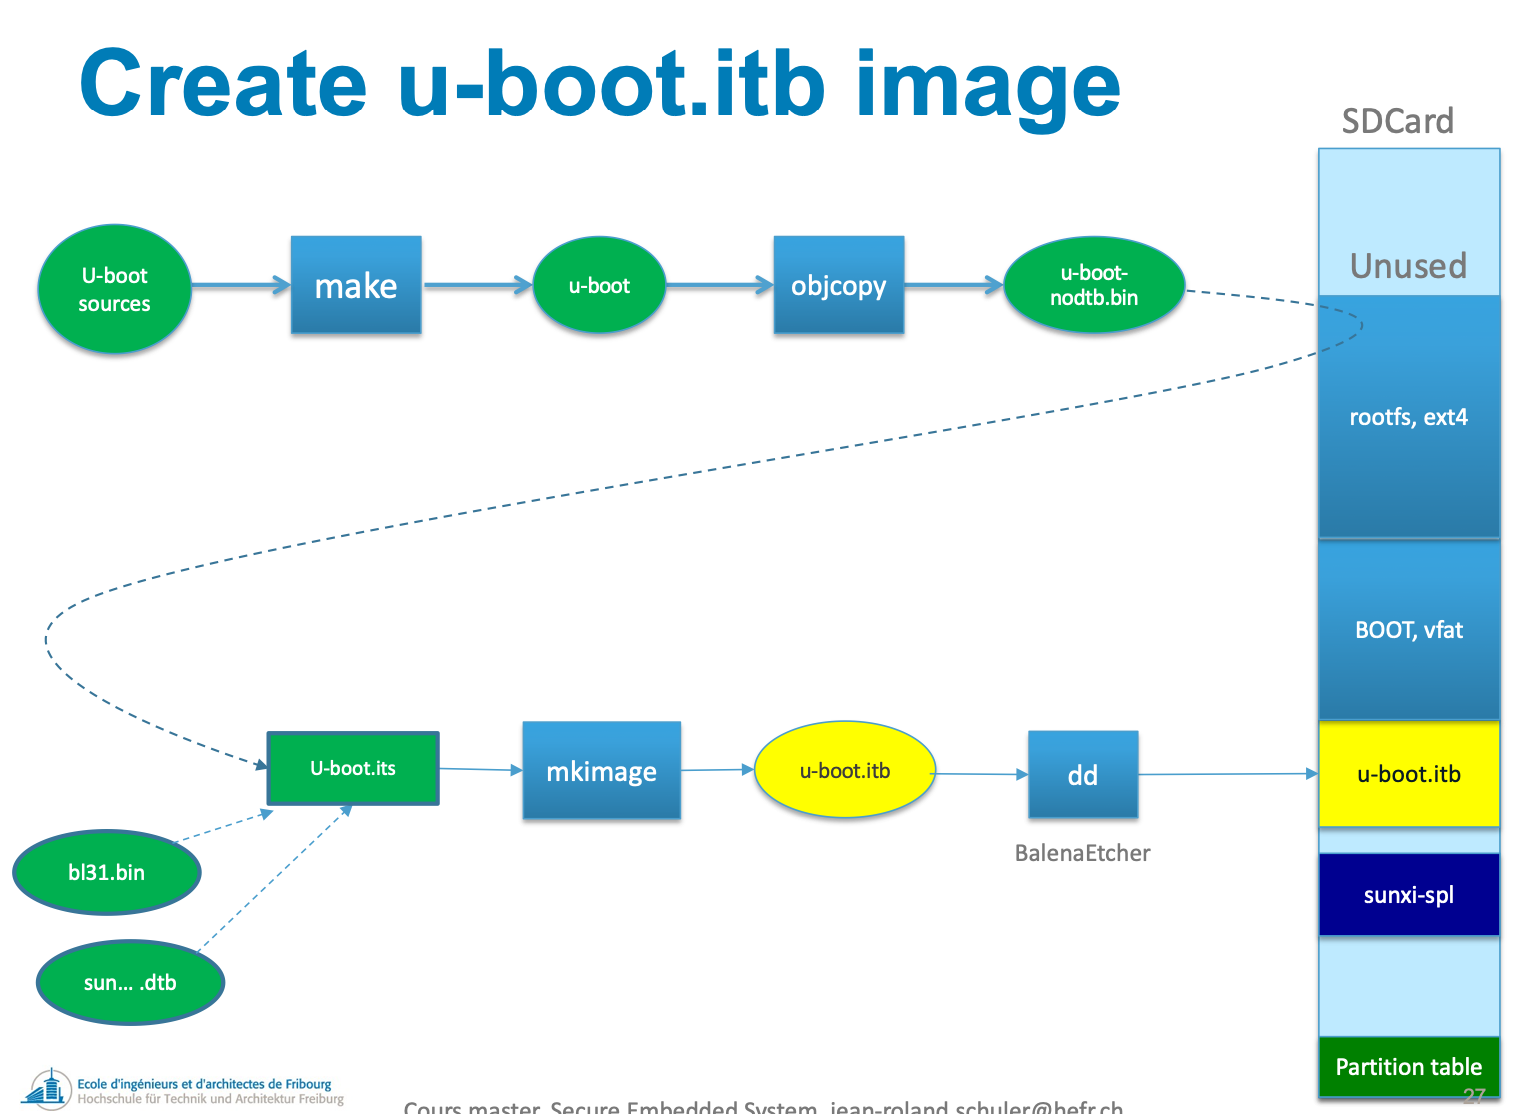
\includegraphics[width=\linewidth]{u-boot_itb.png}
\end{figure}
% ----------
\subsection{FDT (Flattened Device-Tree)}
Le FDT contient une description hardware du système utilisée par Linux pour sa configuration (infos sur le port série, le processeur, etc.). le FDT utilise deux fichiers :
\begin{itemize}
\item \verb!.dts! : Device Tree Source (fichier ascii)
\item \verb!.dtb! : Device Tree Blob (fichier binaire)
\end{itemize}
La commande \verb!dtc! permet de passer de \verb!.dts! à \verb!.dtb!.

Le FDT est stocké dans le fichier \verb!u-boot.itb!
% ----------
\subsection{FIT (Flattened Image Tree)}
Nouveau format qui permet d'insérer plusieurs fichiers dans un seul :
\begin{figure}[H]
    \centering
    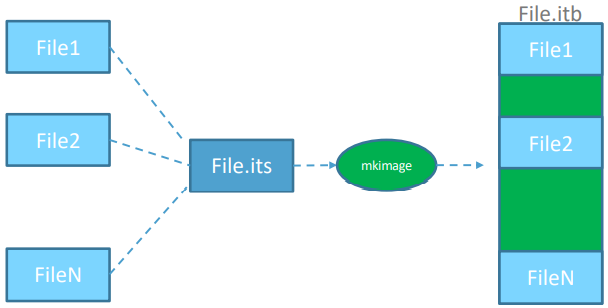
\includegraphics[width=0.75\columnwidth]{FIT.png}
\end{figure}
La commande \verb!mkimage! permet de convertir un fichier \verb!.its! (ascii) en un fichier \verb!.itb! (binaire).

\begin{figure}[H]
    \centering
    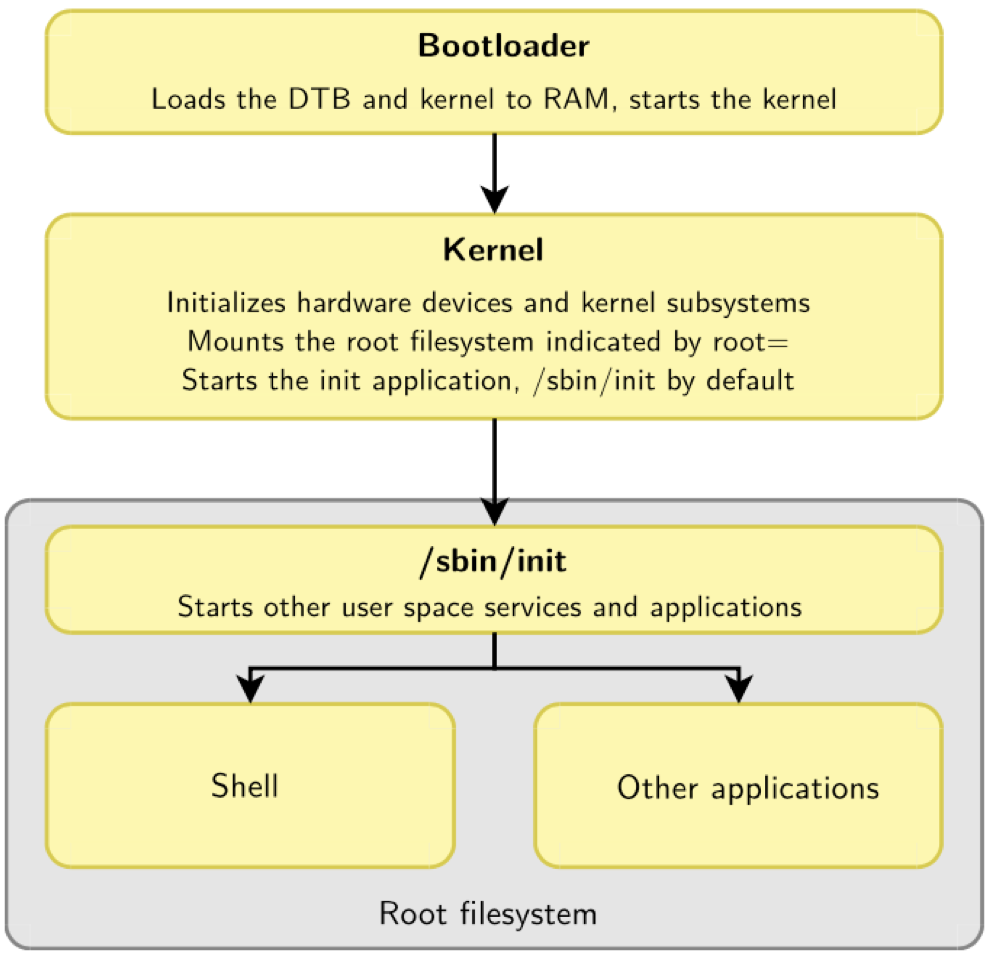
\includegraphics[width=0.8\linewidth]{start_nanopi.png}
\end{figure}

% ----------
\subsection{Séquence de démarrage (6 phases)}

\begin{enumerate}
\item Lorsque le $\mu$P est mis sous tension, le code stocké dans son BROM va charger dans ses 32KiB de SRAM interne le firmware \verb!sunxi-spl! stocké dans le secteur no 16 de la carte SD / eMMC et l’exécuter. 
\item Le firmware \verb!sunxi-spl! (Secondary Program Loader) initialise les couches basses du $\mu$P, puis charge l'U-Boot dans la RAM du $\mu$P avant de le lancer.
\item L'U-Boot va effectuer les initialisations hardware nécessaires (horloges, contrôleurs, …) avant de charger l’image non compressées du noyau Linux dans la RAM, le fichier \verb!Image!, ainsi que le fichier de configuration FDT (flattened device tree).
\item L'U-Boot lancera le noyau Linux en lui passant les arguments de boot (bootargs)
\item Le noyau Linux procédera à son initialisation sur la base des bootargs et des éléments de configuration contenus dans le fichier FDT (sun50i-h5-nanopi-neo plus2.dtb).
\item Le noyau Linux attachera les systèmes de fichiers (rootfs, tmpfs, usrfs, …) et poursuivra son exécution.
\end{enumerate}

\subsubsection{Chargement du Kernel}
\verb+mkimage+ : \verb+boot.cmd+ $\rightarrow$ \verb+boot.scr+

\begin{figure}[H]
    \centering
    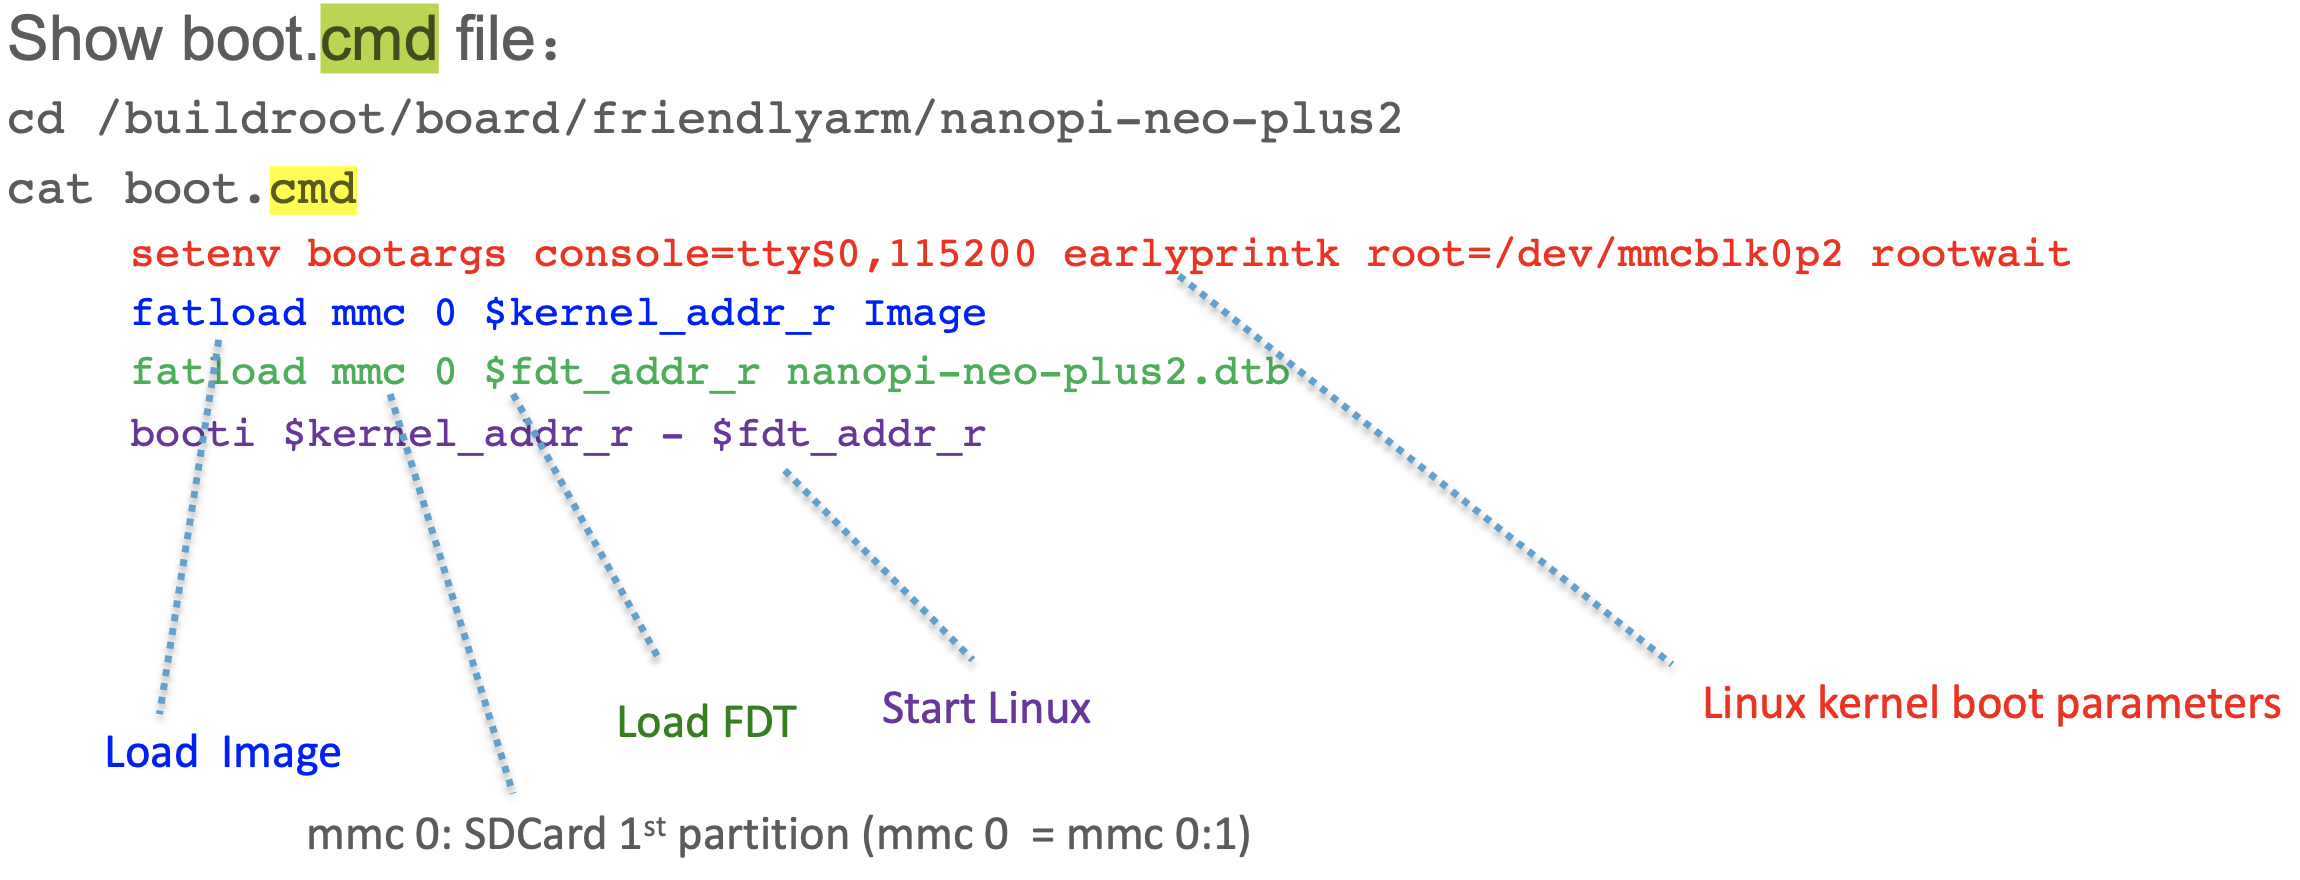
\includegraphics[width=\linewidth]{load_kernel.png}
\end{figure}

\verb+fatload+ charge les images en RAM\\
\verb+booti+ start le kernel en lui donnant l'adresse du kernel et l'adresse du FDT.

\begin{figure}[H]
    \centering
    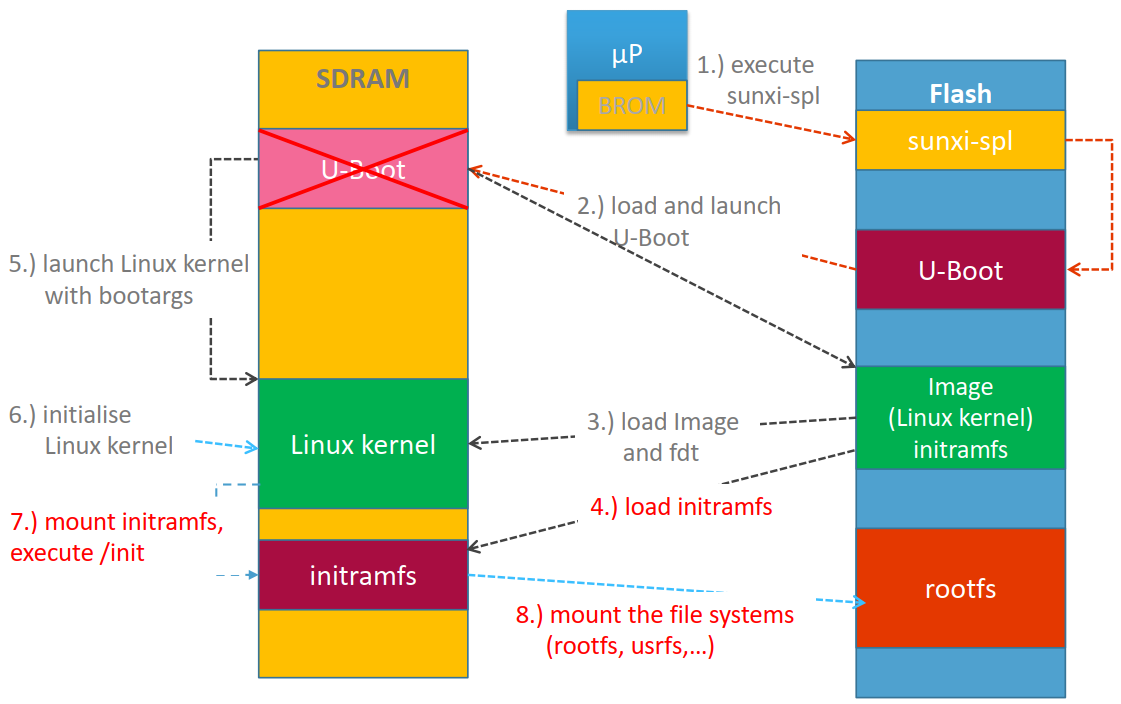
\includegraphics[width=.9\columnwidth]{initRamFsBootSeq.png}
    \label{fig:initRamFsBootSeq}
\end{figure}
\begin{figure}[H]
    \centering
    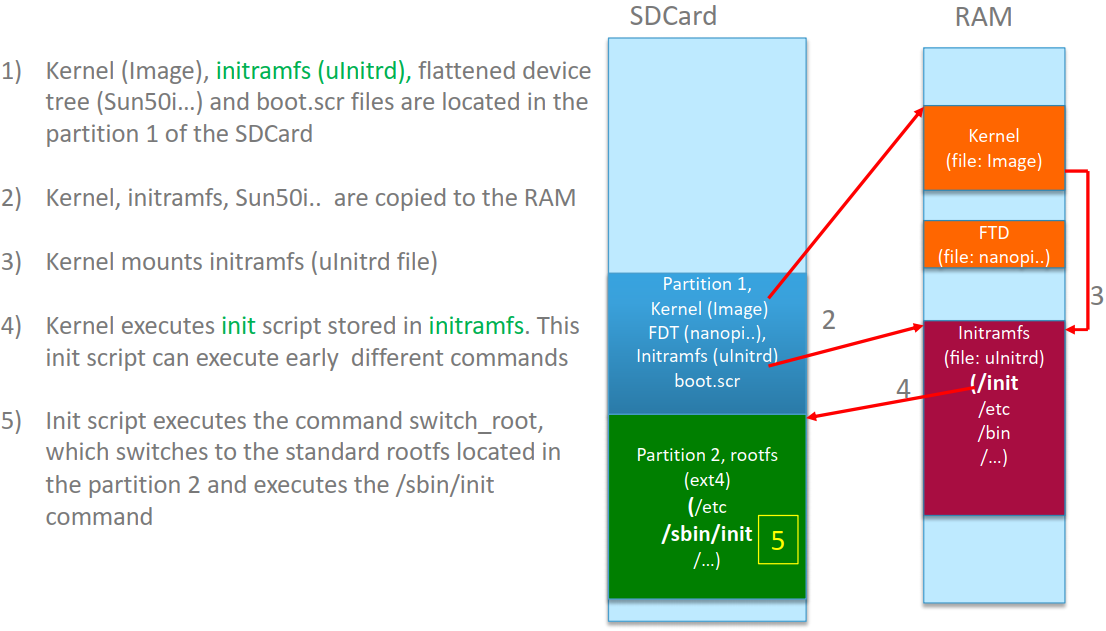
\includegraphics[width=.9\columnwidth]{initRamFsBootSeq2.png}
    \label{fig:initRamFsBootSeq2}
\end{figure}
%\begin{figure}[H]
%    \centering
%    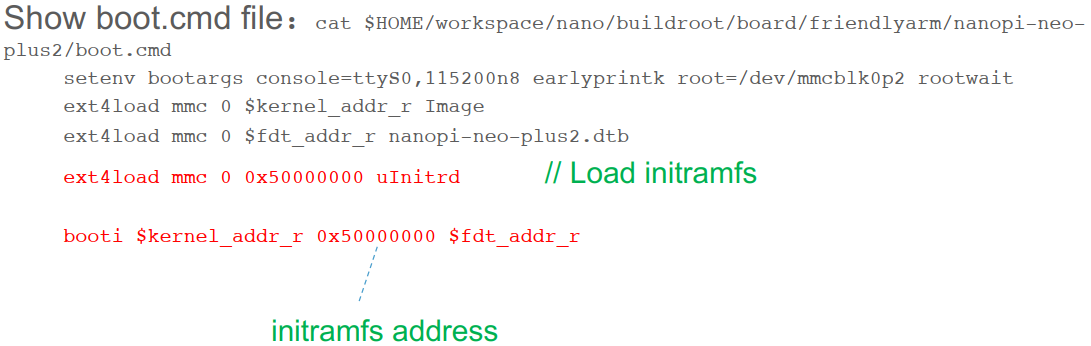
\includegraphics[width=1\columnwidth]{initRamFsBootSeq3.png}
%    \label{fig:initRamFsBootSeq3}
%\end{figure}
\begin{figure}[H]
    \centering
    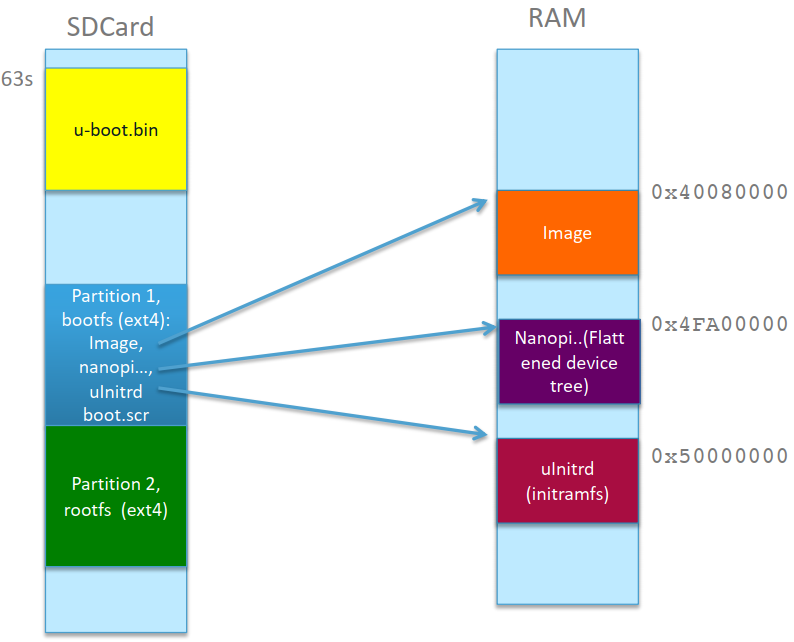
\includegraphics[width=.9\columnwidth]{initRamFsBootSeq4.png}
    \label{fig:initRamFsBootSeq4}
\end{figure}